\documentclass[11pt,a4paper, 
swedish,english %% Make sure to put the main language last!
]{article}
\pdfoutput=1

%% Andréas's custom package 
%% (Will work for most purposes, but is mainly focused on physics.)
\usepackage{../custom_as}

%% Figures can now be put in a folder: 
\graphicspath{ {figures/} %{some_folder_name/}
}

%% If you want to change the margins for just the captions
\usepackage[font=small]{caption}

%% To add todo-notes in the pdf
\usepackage[%disable  %%this will hide all notes
]{todonotes} 

%% Change the margin in the documents
\usepackage[
%            top    = 3cm,              %% top margin
%            bottom = 3cm,              %% bottom margin
%            left   = 3cm, right  = 3cm %% left and right margins
]{geometry}


%% If you want to chage the formating of the section headers
%\renewcommand{\thesection}{...}
\swapcommands{\Lambda}{\varLambda}
\swapcommands{\Omega}{\varOmega}
\swapcommands{\Gamma}{\varGamma}
\newcommand{\Lsq}[1]{\ensuremath{\mathcal{L}^2_{#1}}}
\newcommand{\RT}{\ensuremath{R_{\text{T}}}}
\newcommand{\RH}{\ensuremath{R_{\text{H}}}}
\newcommand{\tf}{\ensuremath{\tilde{f}}}

%%%%%%%%%%%%%%%%%%%%%%%%%%%%%%%%%%%%%%%%%%%%%%%%%%%%%%%%%%%%%%%%%%%%%%
\begin{document}%% v v v v v v v v v v v v v v v v v v v v v v v v v v
%%%%%%%%%%%%%%%%%%%%%%%%%%%%%%%%%%%%%%%%%%%%%%%%%%%%%%%%%%%%%%%%%%%%%%


%% If you want to use an external file for the title page
%\input{titlepages.tex}


%%%%%%%%%%%%%%%%%%%% vvv Internal title page vvv %%%%%%%%%%%%%%%%%%%%%
\begin{titlepage}
\title{\tt Project lambda}
\author{Niklas Renström\footnote{\href{mailto:nikren@student.chalmers.se}{\tt nikren@student.chalmers.se}} 
\and Andréas Sundström\footnote{\href{mailto:andsunds@student.chalmers.se}{\tt andsunds@student.chalmers.se}}
}

\date{\today}

\maketitle


%% Page numbering:
%\pagenumbering{roman} %% roman pagenumbering
\thispagestyle{empty} \pagestyle{empty} %% no page numbers 

%% The abstract of the document
\begin{abstract} 
In this paper we have played around with operators and Bessel functions. It was fun. Thanks for the money Barncancerfonden.
\todo[inline]{Write better abstract, change title, read through and improve language}
\end{abstract}
\newpage
\tableofcontents
\end{titlepage}

\pagenumbering{arabic}
\setcounter{page}{1}
%%%%%%%%%%%%%%%%%%%% ^^^ Internal title page ^^^ %%%%%%%%%%%%%%%%%%%%%
%% If you want a list of all todos
%\todolist


\section{Introduction}

The current hyperthermia treatments mainly utilizes signals consisting of narrow band (NB) signals since simulations and numerical studies have not shown an increase of efficacy by using a wide band (WB). 
However, there exists a number of uncertainty principels stating that a function cannot be highly localized in the space and frequency domains at the same time. This would suggest the use of a wide band of frequencies, in contrast to prior studies.

This project aims to shed some light on this apparent inconsistency by taking a closer look at relevant uncertainty principles and applying them to a simplified case of scalar fields satisfying the wave equation in two dimensions.
First the Heisenberg inequality, a lower limit of the product of the field's variance in the two domains will be applied.
Next, to get something more related to hyperthermia treatment a mathematical framework originally developed by Slepian et al., which speaks of how well a function limited in frequency can be localized in a bounded region of space. 

The main results show that it \emph{is} possible to obtain a localization of the E field with a single frequency but it is greatly enhanced with a WB signal. However as is discussed in Section~\ref{sec:SAR} the increased localization for WB signals does not apply to hyperthermia treatment. 

%Finally the results will be discussed from a hyperthermia treatment point of view and we will discuss some of the limitations as well as possible extensions of the theory.


\subsection{Limitations}
The human body contains many different materials and therefore a real hyperthermia treatment planning will often involve numerically solving Maxwell's equations to simulate how the E field will look in each specific case.

Since this project aims to extract what limitations the \emph{wave nature} sets, we are not concerned with the actual wave propagation -- instead we ask the question, given a perfect way to create or propogate the E field, what limits does a narrow band of frequencies and the wave equation set on the optimal distribution in a bounded region?

With this in mind the study is limited to a homogeneous material stretching through all space. The material is assumed loss-less. %, although the case of lossy materials and dampened E field's will be discussed briefly in Section~\ref{sec:SAR}.
Further we limit ourselves to 2 dimensions since this suffices to capture the essential wave nature in higher dimensions whilst not overly complicating the mathematics. 
In this space we try to focus the distribution to a simple body, a disc since we believe that most more complicated bodies would yield approximately the same results.

%We will also limit our attention to scalar fields, real E fields are in fact vectors with certain limitations to its directions which would produce slightly tighter bounds then what we achieved but this was unfortunately beyond the scope of this project.

Finally, for a real hyperthermia treatment it is not the intensity of the E field that is of concern but rather its mean-value in time that is of interest. This has significant implications for the frequency dependence of the effectiveness of the treatment, and will be discussed at some length in Section~\ref{sec:SAR}. However, the main part of this work is concerned with the E field itself and not its time mean.


\subsection{Theory}
For each frequency $\omega$ the electric field will have a harmonic timedependence,and can be represented by phasor notation,
\begin{equation}
  \label{eq:phasor}
\vb*E(\vb*x,t)=\Re\qty[\vb*E(\vb*x)\ee^{-\ii\omega t}]%\cos(\omega t).
\end{equation}
In a loss-less and source-less homogeneous media the Maxwell equations reduce to
\begin{equation}
\begin{cases}
\laplacian  \vb*E + k^2\vb*E=0,\\
\div\vb*E = 0,
\end{cases}
\end{equation} 
where $k^2 = \omega^2/v^2$ with $v=\frac{1}{\sqrt{\mu \epsilon}}$ being the speed of propagation. 

To simplify matters however, we will limit the scope of this project to scalar fields only satisfying the Helmholtz equation
\begin{equation}
  \label{eq:Helmholtz}
  \qty(\laplacian + k^2)E=0.
\end{equation} 

\subsubsection{Plane wave decomposition}
One solution to the Helmoholtz equation \eqref{eq:Helmholtz} are the plane waves
\begin{equation}\label{eq:plane-wave}
E(\vb*x)=A \ee^{\ii\vb*k \cdot \vb*x},
\end{equation}
were the wavevector $\vb*k$ is any vector such that $\vb*k\vdot\vb*k=k^2$, and $A$ is a constant amplitude. 

The next step is to allow more for more than one frequency. The solution for each frequency will be of the form \eqref{eq:plane-wave}, each with its own amplitude $A(\vb*k)$. These solutions can then be summed up over all frequencies (magnitude as well as directions of $\vb*k$) and the final $E$ field becomes\footnotemark{}
\begin{equation} \label{eq:FT-inv}
E(\vb*x)= (2\pi)^{-D} \oldint_{\vb*k} \rd^Dk\,
A(\vb*k) \ee^{\ii\vb*k\vdot\vb*x}.
\end{equation}
\footnotetext{The factor of $(2\pi)^{-D}$ is just for convenience in the comparison with the $D$ dimensional Fourier transform.}

We can now identify \eqref{eq:FT-inv} as an inverse Fourier transform
of $A(\vb*k)$, and thus $A(\vb*k)$ has to be the Fourier transform of
$E(\vb*x)$:
\begin{equation}\label{eq:FT}
A(\vb*k) = \oldint_{\vb*x} \rd^Dx\, E(\vb*x)\ee^{-\ii \vb*k\vdot\vb*x}.
\end{equation}


\subsubsection{Polar wave decomposition in 2 dimensions}
The 2 dimensional Helmholtz equation \eqref{eq:Helmholtz} in polar cooridnats is
\begin{equation}
\label{eq:Helmholtz_polar}
\qty(\pdv[2]{r}+\frac{1}{r}\pdv{r}+\frac{1}{r^2}\pdv[2]{\theta})E+k^2E=0,
\end{equation} 
Which has the standard non-singular solution
\begin{equation} \label{eq:polar_wave}
E(r, \theta)=\sum_{n=-\infty}^{\infty} a_nJ_n(kr)\ee^{\ii n \theta}.
\end{equation}

Analogously to the plane wave decomposition, we now introduce a spectrum of frequencies, and obtain
\begin{equation}
\label{eq:polar_wave_general}
E(r,\theta)
=\oldint_{k} \rd k \sum_{n=-\infty}^{\infty}\!\!a_n(k) J_n(kr)\ee^{\ii n \theta}
=\sum_{n=-\infty}^{\infty}\!\! \ee^{\ii n \theta} \oldint_{k} \rd{k}\,k\,b_n(k) J_n(kr),
\end{equation}
where in the last step $a_n(k)$ has been replaced with $k\,b_n(k)$ for later convenience.



\section{Localization measures and limits} \label{sec:measures}
To start talking about focusing waves, one has to be able 
to quantify how localized it is. This is mainly done through
different measures on the energy distribution of the wave,
$\abs{f}^2$. 

This report will mainly deal with the fraction of energy in a bounded
area, which was used by
Slepian, Pollack and Landau (SPL) in a series of papers 
\cite{PSWF-I_1961,PSWF-II_1961,PSWF-III_1962,PSWF-IV_1964,PSWF-V_1978}.
However, to address the Heisenberg uncertainty principle, which
concerns a type of variance measure, an account of both types of
measures and how they are used will be given in this section. 


\subsection{Heisenberg's uncertainty principle}
The common quantum mechanical version of Heisenberg's uncertainty
principle states that \emph{the product of the variance of
  position and momentum must be greater than some fixed value}. This
is rooted in the interpretation that position and momentum are
related through fourier transfrom. 

The general mathematical statement of the Heisenberg uncertainty
principle, for a function $f$ and its Fourier transfrom\footnotemark{}
$\tf$, is \cite{Folland} 
\footnotetext{With the Fourier transform defined as in \eqref{eq:FT}. }
\begin{equation} \label{eq:heisenberg}
\Delta_{\vb*a}f \Delta_{\vb*\alpha} \tf \geq \frac{D^2}{4} \quad 
%\forall \vb*a, \vb*\alpha, 
\forall f \in \Lsq{\infty},%[\mathbb{R}^2],
\end{equation}
where $\Delta_{\vb*a}f$ is a variance measure of $f$ is around
\emph{any} reference point $\vb*a$, analogously for
$\Delta_{\vb*\alpha}\tf$ and $\vb*\alpha$.
These variances are defined by
\begin{equation} \label{eq:spread_def}
\Delta_{\vb*a}f=
\frac{\oldint_{\vb*x}\rd^Dx\,\abs{\vb*x-\vb*a}^2\abs{f(\vb*x)}^2}
{\oldint_{\vb*x}\rd^Dx\,\abs{f(\vb*x)}^2},
\end{equation}
and analogously for the Fourier transfrom.


If $\Delta_{\vb*a}f$ is high, $f$ cannot be highly localized to one
single small neighbourhood in space. It does not however, preclude $f$
from having narrow peaks; there can exist several narrow peaks which
are spread out from each other and still have $\Delta_{\vb*a}{f}$
being large. 
For hyperthermia treatment, this means that the variation measure at
best gives a hint on what we want. It is possilbe to achieve a very
strong and narrow radiation peak inside the tumour without violating
the Heisenberg inequality, i.e. using NB signals, as long as a
significant part of the radiation intensity is located outside of the 
head.  
This is a consequence of the particular localization measure used in
the Heisenberg uncertainty relation. It is still a mathematical truth,
but it might be too blunt to be practically applicable in hyperthermia
treatments. 



\subsection{The Slepian-Pollack-Landau method}
\label{sec:SPL-method}
Another localization measure was used by SPL in
\cite{PSWF-I_1961,PSWF-II_1961,PSWF-III_1962,PSWF-IV_1964,PSWF-V_1978}. 
\todo{Maybe change?}
In what follows we will show the broad strokes for developing this
theory. In doing so we will prove the existance of a useful set of
functions ${\psi_i}$ which span the room of frequency-limited
functions.

A square-integrable function $f$ of $D$ variables is said to be
$\Omega$-limited if it can be represented as a Fourier integral over
the bounded region $\Omega$, 
\begin{equation}\label{eq:freq-lim}
f(\vb*x)=\qty(2\pi)^{-D}\oldint_\Omega \rd^Dk\,
\tf(\vb*k)\ee^{\ii(\vb*k \cdot \vb*x)} 
\end{equation}
i.e. it only contains frequencies in the area $\Omega$.


The energy of a function $f$ in a region $S$ is defined as 
\begin{equation}\label{eq:AS}
A_S=\oldint_S\rd^Dx\,\abs{f(\vb*x)}^2.
\end{equation}
Using Parseval's formula, the total engergy of the $\Omega$-limited
function $f$ can be written as 
\begin{equation}\label{eq:Atot}
A=\oldint_{R^D}\rd^Dx\, \abs{f(\vb*x)}^2 =
(2\pi)^{-D}\oldint_\Omega\rd^Dk\, \abs{\tf(\vb*k)}^2.
\end{equation}


By substituing \eqref{eq:freq-lim} into \eqref{eq:AS}, we get
\begin{equation}\label{eq:AS-KS}
\begin{aligned}
A_S%=\oldint_S\abs{f(\vb*x)}^2\id^Dx
&=\qty({2\pi})^{-2D} \oldint_S\rd^Dx \oldint_\Omega \rd^Dk\,
\tf(\vb*k)\ee^{\ii\vb*k\cdot \vb*x}
\oldint_\Omega \id^Dk'\,
\tf^*(\vb*k')\ee^{-\ii\vb*k'\cdot \vb*x}\\
&=\qty (2\pi)^{-D} \oldint_\Omega\rd^Dk\oldint_\Omega\rd^Dk'\,
\tf(\vb*k)\tf^*(\vb*k')K_s(\vb*k-\vb*k')\\
%&=\ip{I\tf}{\tf}
\end{aligned}
\end{equation}
where
\begin{equation} \label{eq:kernel}
K_s(\vb*k-\vb*k')=(2\pi)^{-D}\oldint_S\rd^Dx\,
\ee^{\ii\vb*x \cdot(\vb*k-\vb*k')},
\end{equation}
is called an integral \emph{kernel}.
Define an integral operator $I_S$:
\begin{equation} \label{eq:int_op}
\qty[I_S g](\vb*k')=\oldint_\Omega\rd^Dk\, 
K_S(\vb*k-\vb*k')g(\vb*k).
\end{equation}
The fraction of energy that the $\Omega$-limited function $f$ can have
in a region $S$ can then be written as 
\begin{equation} \label{eq:energy_frac_final}
\frac{A_s}{A}=
\frac{\oldint_\Omega\rd^Dk\, \qty[I\tf](\vb*k)\tf^*(\vb*k)}
{\oldint_\Omega \rd^Dk\, \abs{\tf(\vb*k)}^2}
=\frac{\ip{I_S\tf}{\tf}}{\ip{\tf}},
\end{equation}
where we have defined an inner product on the $\Omega$-space:
\begin{equation} \label{eq:in_prod}
\ip{f}{g} =\oldint_\Omega\rd^Dk\, f(\vb*k)g^*(\vb*k).
\end{equation}


It can be shown that the integral operator \eqref{eq:int_op} is 
self-adjoint and compact. From the Spectral theorem it now follows
that the functions fullfilling the eigenvalue equation 
\begin{equation}
  \label{eq:eigen}
\qty[I_S\psi](\vb*k)=\oldint_\Omega \rd^Dk'\,K_s(\vb*k')\psi(\vb*k') 
=\mu \psi(\vb*k)
\end{equation}
form an orthogonal base for the space $\Omega$. 
It also follows that the maximum of equation
\eqref{eq:energy_frac_final} is
the largest eigenvalue $\mu_0$ of equation \eqref{eq:eigen}. In
other word $\mu_0$ is an upper bound for the fraction of erergy
in $S$ for an $\Omega$-limited function. 
This upper bound will be dependent on the geometries of the areas
$S$ and $\Omega$. The following section will be devoted to calculating
this $\mu_0$ for bandwidth limited function in two dimensions. 



\section{An example with bandwidth-limited fields in two dimensions}

Generating an electric field with a signal with frequencies ranging from $\omega_{\min}$ to $\omega_{\max}$\footnotemark{} corresponds to only allowing nonzero amplitudes for $k$ between a corresponding
$k_{\min}$ and $k_{\max}$ in the expressions for the $E$-field \eqref{eq:FT-inv} and \eqref{eq:polar_wave_general}.
This implies that the plane wave representation (or Fourier transform) of the field only
has values on a spherical shell of inner radius of $k_{\min}$ and outer radius $k_{\max}$.
We denote $k_{\max}$ by $\Gamma$ and $k_{\min}$ as a fraction of this, $k_{\min}=q\Gamma$, with
$q \in [0,1)$ to simplify the calculations.
  \footnotetext{We call such a field bandwidth-limited.}

For the SPL method we wish to limit the field in space to a region $S$. We will study fields in two dimensions and
with the rotational symmetry of Helmholtz equation in mind we choose the simplest of all regions, a disk with radius $R_S$.


\subsection{The SPL method using Fourier transforms}
%\todo[inline]{Move most of the math here to appendix!}
The methodology used here is a direct translation of the ones used in
\cite{PSWF-I_1961} and \cite{PSWF-IV_1964} to $S$ and $\Omega$. This
section will be somewhat short and superficial; this is due to the
fact that the next method will be much more efficient
numerically. Althogh there are some useful tools which will be
developed here.


From the definition of the kernel $K_s$ in equation \eqref{eq:kernel}, we get 
\begin{equation}
K_S(\vb*k-\vb*k') = (2\pi)^{-2}
\oldint_S \rd^2r \ee^{\ii\vb*r\vdot(\vb*k-\vb*k')}.
\end{equation}
By substituting to polar coordinates and using the usual Bessel
function expansion \cite[formula 8.551.4b]{Gradshteyn-Ryzhik} 
\begin{equation}
\ee^{\ii z\cos\theta} = \sum_{m=-\infty}^\infty
\ii^mJ_m(z)\ee^{\ii m\theta}
\end{equation}
and some other Bessel function identities 
\cite[formula~8.472.3]{Gradshteyn-Ryzhik}, we eventually end up with
\begin{equation}\label{eq:KS-short}
K_S(\vb*k-\vb*k') 
=(2\pi)^{-1}R_S\, \frac{J_1(R_S\Delta{k})}{\Delta{k}}.
\end{equation}
With the law of cosines
$\Delta{k}=\abs{\vb*k-\vb*k'}=\sqrt{k^2+{k'}^2-2kk'\cos(\Delta\theta)}$,
where $k=\abs{\vb*k}$, $k'=\abs{\vb*k'}$ and
$\Delta\theta=(\theta-\theta')$ is the angle between $\vb*k$ and
$\vb*k'$.

The numerical method described in Appendix~\ref{apx:num} can only be
applied to 1 dimensional integrals.
To reduce the eigenvalue equation \eqref{eq:eigen} to this form, first
note that $K_S(\vb*k-\vb*k')$ is $2\pi$-periodic in $\Delta\theta$,
and thus has a Fourier series expansion  
\begin{equation} \label{eq:KS-FS}
K_S(k, k', \Delta\theta)  
=\sum_{n=-\infty}^\infty a_{n}(k, k')\, \ee^{\ii n\Delta\theta}
=\sum_{n=-\infty}^\infty \ee^{\ii n\theta}\,a_{n}(k, k')\,\ee^{-\ii n\theta'},
\end{equation}
where 
\begin{equation} \label{eq:KS-FS-coef}
a_{n}(k, k') = \frac{1}{2\pi} \int_0^{2\pi} \rd(\Delta\theta)\; 
K_S(k, k', \Delta\theta)\ee^{-\ii n\Delta\theta}.
\end{equation}
Viewing \eqref{eq:eigen} as the definition of $\psi$, we also know
that the eigenfunctions, $\psi$, has to be periodic in 
$\theta$ since the kernel is periodic in $\theta$. Therefore
$\psi(k, \theta)$ also has to have a Fourier series 
\begin{equation}\label{eq:psi-FS}
\psi(k, \theta) = \sum_{m=-\infty}^\infty b_m(k)\ee^{\ii m\theta}.
\end{equation}
Substituting \eqref{eq:KS-FS} and \eqref{eq:psi-FS} into
\eqref{eq:eigen}, using polar coordinates and changing the order of
summation and integration, yields
\begin{equation}
\mu\sum_{l=-\infty}^\infty b_l(k)\ee^{\ii l\theta}
= \sum_{n=-\infty}^\infty \ee^{\ii n\theta} \sum_{m=-\infty}^\infty 
\int_{q\Gamma}^\Gamma\rd{k'}\,k' a_n(k, k') b_m(k')
\int_{0}^{2\pi}\rd\theta'\,
\ee^{\ii (m-n)\theta'}.
\end{equation}
The $\theta'$ integral is only non-zero when $(m-n)=0$ and
then the integral is just $2\pi$. We now get
\begin{equation}
\mu\sum_{l=-\infty}^\infty b_l(k)\ee^{\ii l\theta}
= 2\pi\sum_{n=-\infty}^\infty \ee^{\ii n\theta} 
\int_{q\Gamma}^\Gamma\rd{k'}\,k' a_n(k, k') b_n(k').
\end{equation}
By the uniqueness of Fourier series expansions, for all non-zero $b_n$
we finally obtain a one dimensional eigenvalue equation
\begin{equation}
\label{eq:eigen_fourier_coef}
\mu_n b_n(k) = 2\pi\int_{q\Gamma}^\Gamma\rd{k'}\,k' a_n(k, k') b_n(k'),
\end{equation}
where $\mu$ has been denoted by $\mu_n$ since each $b_n(k)$
will have a different eigenvalue satisfying
\eqref{eq:eigen_fourier_coef}.  

There is one last thing we can do to make
\eqref{eq:eigen_fourier_coef} more suitable for numerical solution,
and that is to symmetrisize the kernel $k'a_n(k, k')$. To do that we
make the substitution $b_n(k)=\phi_n(k)/\sqrt{k}$, which yields
\begin{equation}\label{eq:eig-n}
\mu_n \phi_n(k) = 2\pi\int_{q\Gamma}^\Gamma\rd{k'}\,
\sqrt{kk'}a_n(k, k') \phi_n(k').
\end{equation}
This makes the kernel $\sqrt{kk'}b_n(k, k')$ symmetric in $k$ and
$k'$, since $b_n(k, k')=b_n(k', k)$ was already symmetric. Besides
making the numerical eigenvalue calculation more efficient, this also
has some nice mathematical implications, for instance $\phi_n$
constitutes an orthogonal base on $[q\Gamma, \Gamma]$.

However, the problem with this method is that the Fourier coefficients
of the kernel, $b_n(k, k')$, cannot be calculated analytically by
direct integration using standard methods. This results in very costly
numerical calculations since $b_n(k, k')$ has to be calculated
numerically for each pair of $k$ and $k'$, on top of then calculationg
the eigenvalues. 
This problem stems from trying to adobt a plane wave decomposition to
polar coordinates. By starting from the polar wave decomposition one
can avoid these difficulties, which is what we will do in the
following section. 


\subsection{Expanding the SPL method using Bessel decomposition}
The SPL method can be expanded to also cover polar decomposition
\eqref{eq:polar_wave_general}. The main idea of this generalization is
that for circularly symmetric geometries in 2D, polar decomposition
using Bessel function is more natural. 
This generalization will here be illustrated through the example using
$S$ and $\Omega$ as defined above, and the goal should be to
circumvent the problem of evaluating \eqref{eq:KS-FS-coef} from the
previous section.

To calculate the energy of the field $E$ in the disk $S$, we
substitute \eqref{eq:polar_wave_general} into \eqref{eq:AS}: 
\begin{equation}
\begin{aligned}
A_S= \int_S \rd^2x\, \abs{E}^2 = 
\int_0^{R_S} r\rd{r} \int_0^{2\pi} \rd\theta \,&
\int_{q\Gamma}^\Gamma \rd{k}\!\!
\sum_{n= -\infty}^{\infty}\!\! kb_n(k) J_n(kr)\ee^{\ii n \theta}\\
&\times
\int_{q\Gamma}^\Gamma \rd{k'}\!\!
\sum_{m= -\infty}^{\infty}\!\! k'b_m^*(k') J_n(k'r)\ee^{-\ii m
  \theta}.
\end{aligned}
\end{equation}
If we now rearrange the order of sumation and integration, and
evaluate the $\theta$ integral, we see that non-vanishing terms are
with $m=n$ and then we get a factor of $2\pi$ like in the previous
section. By introducing the kernel 
\begin{equation}\label{eq:KS-bessel}
K_S^{(n)}(k, k') = \int_{0}^{R_s} \rd{r}\, r J_n(kr) J_n(k'r),
\end{equation}
the energy in $S$ can be written as
\begin{equation}\label{eq:AS-bessel}
A_S =2\pi \sum_{n=-\infty}^{\infty} 
\int_{q\Gamma}^\Gamma \rd{k} \int_{q\Gamma}^\Gamma \rd{k'}\,  
kk'\, b_n(k)b_n^*(k') K_S^{(n)}(k, k')
\end{equation}

If we let the radius $R_S$ of the disk $S$ tend to infinity, and by
using the asymptotic behavior of Bessel functions, the the infinte
kernel can be witten as
\begin{equation}
K_\infty^{(n)}(k,k') = \frac{\delta(k-k')}{k'}.
\end{equation}
This implies that the total energy
\begin{equation}\label{eq:A-bessel}
\begin{aligned}
A &=2\pi \sum_{n=-\infty}^{\infty} 
\int_{q\Gamma}^\Gamma \rd{k} \int_{q\Gamma}^\Gamma \rd{k'}\,  
kk'\, b_n(k)b_n^*(k') \frac{\delta(k-k')}{k'} \\
&=2\pi \sum_{n=-\infty}^{\infty} 
\int_{q\Gamma}^\Gamma \rd{k} \, k\, b_n(k)b_n^*(k).
\end{aligned}
\end{equation}

With \eqref{eq:AS-bessel} and \eqref{eq:A-bessel}, the energy fraction
can be written as
\begin{equation}\label{eq:E-frac-bessel}
\frac{A_S}{A}
=\frac{\displaystyle{\sum_{m}} \int_{q\Gamma}^\Gamma \rd{k} \int_{q\Gamma}^\Gamma \rd{k'}\,  
kk'\, b_m(k)b_m^*(k') K_S^{(m)}(k, k')}
{\displaystyle{\sum_{n}} \int_{q\Gamma}^\Gamma \rd{k} \, k\, b_n(k)b_n^*(k)}.
\end{equation}
By similar arguments as in Section~\ref{sec:SPL-method}, the maximum
of this fraction is given as the largest eigenvalue to
\begin{equation}
\mu_nb_n(k) = \int_{q\Gamma}^{\Gamma}\rd{k}\,k K_S^{(n)}(k, k')\,b_n(k').
\end{equation}
Note that the equation above is different for each $n$, and the
maximum is to be taken over all $n$.

Analagously to the case in the previons section, theis eigenvalue
equation can be symmetrisized to
\begin{equation}\label{eq:eig-n-bessel}
\mu_n\phi_n(k) = \int_{q\Gamma}^{\Gamma}\rd{k}\,
\sqrt{kk'} K_S^{(n)}(k, k')\,\phi_n(k').
\end{equation}
This looks suspiciously similar to \eqref{eq:eig-n} from the previous section, and oin fact since both of these methods concern the same problem, \eqref{eq:eig-n-bessel} and \eqref{eq:eig-n} \emph{are} the same equations, but now we have an analytical expression for $K_S^{(n)}(k, k')$ (see below). The reason for this equivalence can easily be seen if one writes down the 2D Fourier transform, using polar coordinate, of a Fourier series. 

The advantage of this method is that this time, the kernel
\eqref{eq:KS-bessel} can be calculated analytically
\cite[formula 5.54]{Gradshteyn-Ryzhik}
\begin{equation}\label{eq:kernel_expr}
K_S^{(n)}(k, k') =
\begin{cases}
\frac{R_S}{k^2-k'^2}
\qty[k'J_{n}(R_sk)J_{n-1}(R_sk')-kJ_{n-1}(R_sk)J_{n}(R_sk')]
\qc &k\neq k'\\
\frac{R_S^2}{2}\qty[ \qty(J_{n}(R_Sk))^2
-J_{n-1}(R_sk)J_{n+1}(R_sk)]
\qc &k= k'.
\end{cases}
\end{equation}
So now, the numerical calculation of the eigenvalues are significantly
faster than with the previous method.


\subsection{Energy of a single frequency}
It is also of interest to study how much energy a field limited to one frequency
$\omega_i$ can maintain if it is limited to $S$. Starting from equation \eqref{eq:polar_wave}
and using similar arguments as in the previous section one arrives to the expression
\begin{equation}
A_S=2\pi\sum_n \abs{a_n}^2\int_0^{R_S}\rd r \, r (J_n(k_ir))^2,
\end{equation}
where $k_i=\frac{\omega_i}{v}$ as usual.
The integral is recognized as the one defining the kernel $K_S$ for ($k=k'$) and from equation \eqref{eq:kernel_expr} we obtain
\begin{equation}\label{eq:energy_single}
A_S=2\pi \sum_n \abs{a_n}^2\frac{R_S^2}{2}\qty[ \qty(J_{n}(R_Sk_i))^2
-J_{n-1}(R_sk_i)J_{n+1}(R_sk_i)].
  \end{equation}


%%%%%%%%%%%%%%%%%%%%%%%%%%%%%%%%%%%%%%%%%%%%%%%%%%%%%%%%%%%%%%%%%%%%%%
\section{Results}
In this section the localization measures and limits described in section \ref{sec:measures}
have been applied to scalar fields. These fields have been built as a sum of solutions the Helmholtz
equation for different $k$:s in an interval $[k_{\min},\,k_{\max}]$ and are to be seen as representatives
of real electric fields in a lossless media coming from a bandwidth-limited signal.


\subsection{Heisenberg's inequality for bandwidth-limited functions}
A bandwidth-limited field in three dimensions will have a Fourier transform that is located on a spherical
shell. Such a distribution has a maximal variance if all of it lies on the outermost layer. The variance
in the frequencyroom is then given by $\Delta \tf=k_{\max}^2$. Heisenberg's inequality \eqref{eq:heisenberg}
now yields
\begin{equation}
\Delta f \geq \frac{9}{4k_{\max}^2}=\frac{9\lambda_{\min}^2}{16\pi^2}.
\end{equation}
Thus the lowest variation of is only dependent on the shortest wavelength $\lambda_{\min}$ and not on the actual bandwidth.

\subsection{Energy of bandwidth-limited functions in a bounded region}
\begin{figure}\centering
\centerline{ % centers figures larges than 1\textwidth
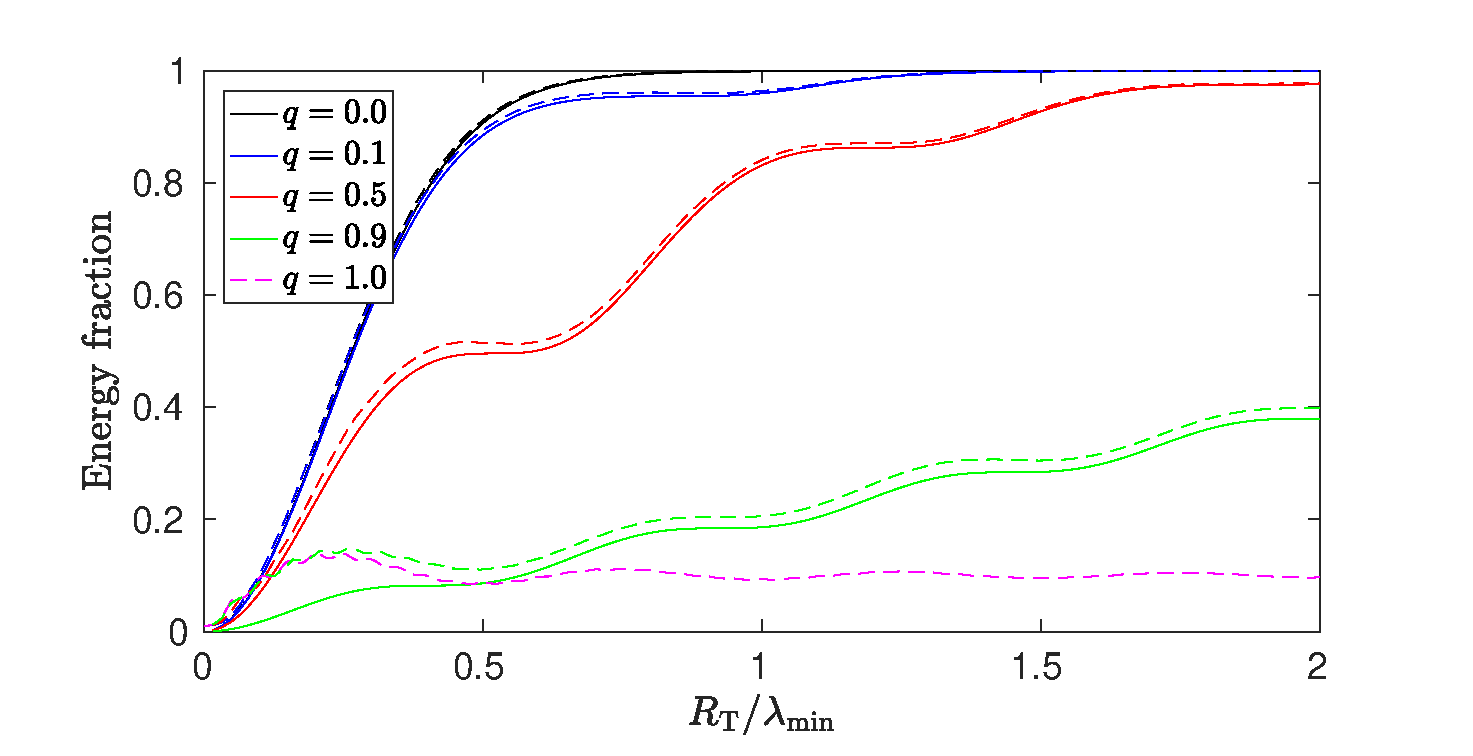
\includegraphics[width=16cm]{ring_both_L1000.eps}
}
\caption{Theoretical maximum of energy fraction inside the tumor for isotropic 
  fields, both compared to the total energy in real space (solid line) as well as
  compared to a ``head'' region (dashed line). The fractions are plotted as
  a function of tumor size, $\RT$, measured in shortest wavelengths,
  $\lambda_{\min}$. The different values of $q\in[0, 1]$ corresponds to 
  the width of the frequency band, where $\lambda_{\min}=2\pi/\Gamma$ and
  $\lambda_{\max}=\lambda_{\min}/q$, i.e. a larger $q$
  means a narrower band. The head and tumor regions used were concentrical discs;
  where the radius of the head region was $10\RT$. }
\label{fig:both}
\end{figure}

In \figref{fig:both} the eigenvalues of \eqref{eq:eig-n-bessel}, with $n=0$, are shown 
for different values of the ratio between the tumour size and the shortest wavelength, $\RT/\lambda_{\min}=\RT\Gamma/(2\pi)$. For $q=1$ the analytical solution \eqref{eq:energy_single} was used while for the other $q$:s the eigenvalues where numerically calculated with the method in Appendix~\ref{apx:num}.
This corresponds to the theoretical maximum of the energy focused in a circularly tumor for isotropic (angularly independent) fields in twodimensions, limited to wavelengths between $\lambda_{\min}$ and $\lambda_{\max}$.
The reason we choose to plot for isotropic fields ($n=0$) is that this corresponded to the largest eigenvalue for most values of $\RT\Gamma$, especially the lower ones.
The different curves correspond to different bandwidth with $q=\lambda_{\min}/\lambda_{\max}$. The solid curves represent the fraction of energy in the tumor region to the whole space ($A_T/A$) while the dashed curves the fraction of energy in the tumor to a ``head'' region ($A_T/A_H$), a ten times larger concentrical disc. These dashed lines do not represent the maximum fraction in the tumor compared to the head, instead they correspond to the functions that maximized $A_T/A$ but this time ``normalized''  to the energy in the head.

For small q-values ($0$, $0,1$) the fractions approach 1 quite quickly and for $\RT$ being half the size of the shortest wavelength and larger it is possible to have almost all the energy located in the tumor. It is also apparant that also the bandwidth plays a significant role for the localization, for $q=0,5$ only about 50\,\% of the energy is focused in a tumor with $\RT=\lambda_{\min}/2$ and for $q=0,9$ less than 10\,\%.
This also explains the relatively small differences between the dashed and solid curves; for small $q$-values focusing in the tumor places apparantly focuses almost all the energy in the head. Intuitively it makes sense that focusing in the head is achieved when focusing in the center of the head and from the figure it is apparant that it \emph{is} possible to focus almost all the energy in a head ten times the tumor for all but the largest $q$:s and smallest $R_T$:s. For large $q$ it does however make a difference by comparing with the head since these fractions does not converge as quickly to 1. 

The figure also clearly shows that, when comparing to the head, it \emph{is} possible to achieve some localization even for a single frequency. For $\RT \approx \lambda_{\min}/4$ one achieves a maximum of approximately 0,15. That is one can focus roughly 15\,\% of the energy in the head to 1\,\% of the area.

%the difference between the dashed and solid lines is very small which signifies that by trying to focus energy in he tumor we 


%%%%%%%%%%%%%%%%%%%%%%%%%%%%%%%%%%%%%%%%%%%%%%%%%%%%%%%%%%%%%%%%%%%%%%
\section{Discussion and outlook}
\todo[inline]{T. Köhler}

%\subsection{The issue of using a wide or narrow frequency band}
%Figure 1 clearly shows that we have faild to prove that NB is good...

This report has only treated some very simplified examples, although the presented SPL technique can still be applied to any general geometry. To three dimensions it can for instance be generalized with the use of spherical Bessel functions and spherical harmonics. For more general geometries the trade-off would however be that more of the calculations would have to be done numerically instead of analytically. 
%The justification however for showing these examples is that they give a theoretically achievable maximum for any field, and thus gives some qualitative insight

Appart from different geometries, it would also be desirable to compare the radiation inside the tumor to the head istead of compared to the total energy of the field.
%The SPL method is based upon maximizing the energy within a bounded region $S$
%compared to the total energy in the room. This is not really the kind of optimization
%one wants to do for a hyperthermia treatment where we are concerned of what happens in the head.
%Therefore a measure of the kind $A_T/A_H$ where $T$ ($H$) stands for the tumor (head) region, would be prefered.
To generalize the measure \eqref{eq:energy_frac_final} to incorporate a head region, the denominator has to be changed to $\ip*{I_\text{H}\tf}{\tf}$, where $I_\text{H}$ is defined analogously to $I_\text{T}$. The generalized problem can be proven to have be optimized by the generlaized eigenvalue problem $I_\text{T} \psi'=\mu I_\text{H}\psi'$. 

Conceptually this should be easily implemented in the numerical method used here. However when we tried to solve the generalized eigenvalue problem the numerics turned out to be badly conditioned due to the head matrices being almost singular. 
Because of this, we instead choose to calculate $A_\text{T}/A_\text{H}$ for the regular eigenvector, $\psi$, of $I_\text{T}$. 

The justification for using the regular eigenvector, instead of the generalized, is that for a head considerably larger than the tumor the regular eigenvalues are almost 1, as seen in \figref{fig:both}. This means that the head then already contains close to all of the energy in the field, which means that the generalized eigenvalue will be almost the same. This is not completely true for the low values of $\RT/\lambda_{\min}$ and high values of $q$. However, in the case with $q=0.9$ the agreement with the (true) optimum for $q=1$ indicates that using the regular eigenfuntion was not detrimental.
%if the head is considerably larger than the tumor, then $I_\text{H}$ will almost be the identity operator. This can clearly be seen in the extreme case when the head becomes the whole space. 

Another overlooked detail is the fact that \figref{fig:both} only presents the values for $n=0$, but to find the real optimum one has to find the largest eigenvalue $\mu_n$ over all $n$. Indeed, when this was investigated numerically we found regions where $n>0$ had a larger energy fraction. However $\mu_0$ was in most cases the largest eigenvalue, and it does give a good representation of what the maximum energy fraction would be.

Despite of not being directly applicable to hyperthermia treatment, these examples gives a theoretically achievable maximum for any field, and can be used for some qualitative insight to how the wave-nature limits the localization of a field. For instance \figref{fig:both} shows that one can focus almost all the energy of the field into a tumor of the same size as the shortest wavelength (highest frequency) if all the longer wavelengths (lower frequencies) are also used. If however the signal is limited to a narrow band of frequencies, not containing the lowest ones, the fraction of energy one can focus in the tumor quickly falls off. For focusing electric field intensity in a bounded region it is therefore prefered to use a wide band signal. But due to an effect of time-averaging this is not true for hyperthermia treatments which will be discussed in the following section.



\subsection{Specific Absorption Rate compared to ntensity}
\label{sec:SAR}
\todo{Rubrik, inledning?}
In hyperthermia treatment a good indicator for the temperature
increase is the Specific Absorption Rate (SAR): 
\begin{equation}
\text{SAR}(\vb*x)=
\frac{\ev{\vb*J(\vb*x,t)\vdot \vb*E(\vb*x,t)}_t}{\rho(\vb*x)},
\end{equation}
where $\vb*J$ is the current density, $\vb*E$ is the
electric field, $\rho$ is the mass density, and $\ev{\xi}_t$ denotes
the time average of some quantity $\xi$.
Due to Ohm's law this is simply a weighted version of the intensity
$I=\abs{\vb*E}^2$.
However, due to the time-averaging, intereference between multiple
frequencies vanishes \cite{Martinsson}. Thus
\begin{equation}
\text{SAR}(\vb*x)=\sum_i\text{SAR}_{\omega_i}(\vb*x),
\end{equation}
that is a sum over the contribution from each frequency.

Due to this linearity, and since a finite enrgy will always be applied, it can be proven from the theory of convex optimization 
that a large family of of goalfunctions, convex goalfunctions, are optimized by using a single frequency only. 
In particular, this applies to any linear goalfunction such as the main goalfunction used in this paper
\eqref{eq:energy_frac_final}. Therefore if it was applied to SAR it would be maximized by a single frequency.  




%%%%%%%%%%%%%%%%%%%%%%%%%%%%%%%%%%%%%%%%%%%%%%%%%%%%%%%%%%%%%%%%%%%%%%
\section{Conclusions}





%%%%%%%%%%%%%%%%%%%%%%%%%% The bibliography %%%%%%%%%%%%%%%%%%%%%%%%%%
%\newpage
%% This bibliography ueses BibTeX
\bibliographystyle{ieeetr}
\bibliography{references}%requires a file named 'references.bib'
%% Citations are as usual: \cite{example_article}

%%%%%%%%%%%%%%%%%%%%%%%%%%%%% Appendices %%%%%%%%%%%%%%%%%%%%%%%%%%%%%
\clearpage %% on a new page 
\appendix  %% This will change the page numbering to A1, A2, A3, ...;
           %% and also change the sections to A, A.1, ...; B, B.1, ...


%%%%%%%%%%%%%%%%%%%%%%%%%%%%%%%%%%%%%%%%%%%%%%%%%%%%%%%%%%%%%%%%%%%%%%
\section{Numerical implementation of the 
Landau-Pollack-Slepian Theory}
\label{apx:num}
In the previous section we have been occupied by integral eigenvalue
equations of the form
\begin{equation} %\label{eq:int-eig}
\mu E(k) 
= \oldint_{\Omega} \rd^D{k}\, K(k, k') E(k')
\qcomma k, k'\in\Omega.
\end{equation}
We have also put down some work to reduce higher-dimensional
integrals to one-dimensional ones
\begin{equation} \label{eq:int-eig}
\mu \psi(k) 
= \oldint_{I} \rd{k}\, K(k, k') \psi(k'),
\end{equation}
where the integration is now over an interval 
$I=[\alpha, \beta]$. This was done so that the numerical method
presented here could be applied. 


\subsection{Discretization of the integral equation}
The integral can be discretized according to
\begin{equation} \label{eq:inttosum}
\begin{aligned}
\oldint_I\rd{k} &\to \sum_{n=1}^N\Delta{k}
=\frac{\abs{I}}{N} \sum_{n=1}^N,\\
\psi(k) \to \psi_n = \psi(k_n) &\qcomma
K(k, k') \to K_{m, n} = K(k_m, k_n),
\end{aligned}
\end{equation}
where $\abs{I}=\beta-\alpha$ is the size of the interval $I$.
With these discretizations, \eqref{eq:int-eig} discretizes to
\begin{equation}
\mu\Psi_m = \frac{\abs{I}}{N} \sum_{n=1}^N K_{m, n} \Psi_n
\end{equation}
which is just a matrix eigenvalue equation
\begin{equation} \label{eq:mtx-eig}
\mu' \Psi = \mathsf{K}\Psi,
\end{equation}
where $\mu'=N\mu/\abs{I}$ and $\mathsf{K}$ is the $N\times N$ matrix
whose element $(m, n)$ is $K_{m, n}$. From here, there are many high
performance linear algebra libraries to find the eigenvalues and
eigenvector to \eqref{eq:mtx-eig} numerically. 

%\subsubsection{Symmetrization }
%We can also
Note that some effort was put into making the integral
kernel symmetric. This not only has the effect of guarateeing that the
eigenvectors of different eigenvalues will be orthogonal, but is also
beneficial to most numerical methods to find eigenvalues. 


% \subsubsection{Physical interpretation}
% An interesting physical interpretation of the discretization is that
% the operation \eqref{eq:inttosum} can be viewed as introducing
% \begin{equation}
% \Delta{k}\qty[\delta(k-k_0) + \delta(k-k_1) +\ldots+\delta(k-k_N)]
% \end{equation}
% into the integral, and effectively limiting the frequencydomain
% $\Omega$ to the dicrete frequencies $k_n$. 

% This idea could possibly be more cloesly related to reality, where the
% differnt antennas only transmitts in certain dicrete frequencies. And
% thus the discretized eigenvalue problem gives the theoretical maximum
% energy in a bounded region in space from a signal restriced to the
% chosen frequencies. 
% It is however worth pointing out that this result has only been proven
% for the 1D case\cite{PSWF-V_1978}, but there is no reason to believ
% that the discetized version cannot be extended to higher dimension
% like in the continuous case. 


\subsection{Verification of the numerical method}
To verify that the method above is sound, we have here compared some calculated eigenvalues for different values of $R_S\Gamma$ to the ones given in \cite{PSWF-IV_1964}. In \tabref{tab:verification}, we see that the relative error (bold) is very small. It is therefore highly likely that the method is sound.


\begin{table}
\centering
\caption{Table of eigevalues to the 2D disc of frequencies, as given
  by Slepian in \cite{PSWF-IV_1964}, $\mu$, and numerically
  calculated using the method of this section, $\hat\mu$; also the
  relative discrepancies between Slepian's method and this is given as
  $(\hat\mu-\mu)/\mu$. The numerical values have been
  calculated using both the algorithem for only the full disc, and
  also using the algorithm for a circle ring with $q=1/L$.
}
\label{tab:verification}
\begin{tabular}{|r|c|c|c|c|c|}\cline{2-6}
\multicolumn{1}{c|}{}
&Slepian\cite{PSWF-IV_1964}&
\multicolumn{2}{|c|}{Disc, numerical ($L=5000$)}&
\multicolumn{2}{|c|}{Ring, numerical ($L=1000$)}
\\ \hline
$R_S\Gamma$\phantom{1.}&$\mu$
&$\hat\mu$&$(\hat\mu-\mu)/\mu$
&$\hat\mu$&$(\hat\mu-\mu)/\mu$
\\ \hline
  0.1 & 2.4968775e-3 & 
2.49787510e-03 &\bf\phantom{-}4.0e-4&  
2.49687188e-03 &\bf-2.3e-6
\\ \hline
  0.5 & 6.0585348e-2 & 
6.06088302e-02 &\bf\phantom{-}3.9e-4&  
6.05834074e-02 &\bf-3.2e-5
\\ \hline
  1.0 & 2.2111478e-1 & 
2.21192655e-01 &\bf\phantom{-}3.5e-4&  
2.21087997e-01 &\bf-1.2e-4
\\ \hline
  1.5 & 4.2951906e-1 & 
4.29646579e-01 &\bf\phantom{-}3.0e-4&  
4.29407932e-01 &\bf-2.5e-4
\\ \hline
  2.0 & 6.2963045e-1 & 
6.29775619e-01 &\bf\phantom{-}2.3e-4&  
6.29363231e-01 &\bf-4.2e-4
\\ \hline
  3.0 & 8.8705036e-1 & 
8.87143325e-01 &\bf\phantom{-}1.0e-4&  
8.86395173e-01 &\bf-7.3e-4
\\ \hline
  5.0 & 9.9534230e-1 & 
9.95350350e-01 &\bf\phantom{-}8.1e-6&  
9.94366440e-01 &\bf-9.8e-4
\\ \hline
 10.0 & 9.9999957e-1 & 
9.99999399e-01 &\bf\phantom{}-1.7e-7&  
9.98997959e-01 &\bf-1.0e-3
\\ \hline
\end{tabular}
\end{table}


%%%%%%%%%%%%%%%%%%%%%%%%%%%%%%%%%%%%%%%%%%%%%%%%%%%%%%%%%%%%%%%%%%%%%%
\end{document}%% ^ ^ ^ ^ ^ ^ ^ ^ ^ ^ ^ ^ ^ ^ ^ ^ ^ ^ ^ ^ ^ ^ ^ ^ ^ ^ ^
%%%%%%%%%%%%%%%%%%%%%%%%%%%%%%%%%%%%%%%%%%%%%%%%%%%%%%%%%%%%%%%%%%%%%%




%%%%  Some (useful) templates


%% På svenska ska citattecknet vara samma i både början och slut.
%% Använd två apostrofer: ''.


%% Including PDF-documents
\includepdf[pages={1-}]{filnamn.pdf} % NO blank spaces in the file name

%% Figures (pdf, png, jpg, ...)
\begin{figure}\centering
\centerline{ % centers figures larges than 1\textwidth
\includegraphics[width=.8\textwidth]{file_name.pdf}
}
\caption{}
\label{fig:}
\end{figure}

%% Figures from xfig's "Combined PDF/LaTeX"
\begin{figure}\centering
\resizebox{.8\textwidth}{!}{\input{file_name.pdf_t}}
\caption{}
\label{fig:}
\end{figure}


%% If you want to add something to the ToC
%% (Without having an actual header in the text.)
\stepcounter{section} %For example a 'section'
\addcontentsline{toc}{section}{\Alph{section}\hspace{8 pt}Labblogg} 

